%%%---PREAMBLE---%%%%%%%%%%%%%%%%%%%%%%%%%%%%
\documentclass[oneside,12pt,final]{sty/ucthesis-CA2012}
\pdfoutput=1

%--- Packages ---------------------------------------------------------
\usepackage[lofdepth,lotdepth,caption=false]{subfig}
\usepackage{fancyhdr}
\usepackage{hyperref}
\usepackage{amsmath, amssymb, graphicx}
\usepackage{xspace}
\usepackage{braket}
\usepackage{color}
\usepackage{setspace}
%\usepackage{subfigure} (Subfigure package clashes with another package)

%---New Definitions and Commands------------------------------------------------------
\def\p{\partial}
\def\im{\mrm{im}}
\def\Tr{\mrm{Tr}}
\def\Z{\mbb{Z}}
\def\R{\mbb{R}}
\def\C{\mbb{C}}
\def\half{\frac{1}{2}}
\def\filler{\phantom{fillerfillerfiller}}
\newcommand{\be}{\begin{equation}}
\newcommand{\ee}{\end{equation}}
\newcommand{\mbb}[1]{\mathbb{#1}}
\newcommand{\mrm}[1]{\mathrm{#1}}
\newcommand{\mcal}[1]{\mathcal{#1}}
\newcommand{\mbf}[1]{\mathbf{#1}}
\newcommand{\ph}[1]{\phantom{#1}}
\newcommand{\udten}[3]{#1^{#2}_{\ph{#2}#3}}
\newcommand{\duten}[3]{#1^{\ph{#2}#3}_{#2}}
\newcommand{\pd}[2]{\frac{\p#1}{\p#2}}
\newcommand{\D}[2]{\frac{d#1}{d#2}}

%---Set Margins ------------------------------------------------------
\setlength\oddsidemargin{0.25 in} \setlength\evensidemargin{0.25 in} \setlength\textwidth{6.25 in} \setlength\textheight{8.50 in}
\setlength\footskip{0.25 in} \setlength\topmargin{0 in} \setlength\headheight{0.25 in} \setlength\headsep{0.25 in}

%%%---DOCUMENT---%%%%%%%%%%%%%%%%%%%%%%%%%%%%
\begin{document}

%=== Preliminary Pages ============================================
\begin{frontmatter}
	\setlength{\droptitle}{-10em}

\pretitle{
  \begin{center}
  University of California, Santa Barbara\\
  \vspace{10em}
}

\title{A semantic typology of lexical flexibility}

\posttitle{
  \\
  \vspace{3.5em}
  A dissertation submitted in partial satisfaction of the requirements for the degree Doctor of Philosophy in Linguistics
  \end{center}
}

\preauthor{
  \begin{center}
  by\\
  \vspace{1em}
}

\author{Daniel W. Hieber}

\postauthor{
  \\
  \vspace{5em}
  Committee in Charge:\\
  Professor Marianne Mithun, Chair\\
  Professor Benard Comrie\\
  Professor Stefan Th. Gries\\
  Professor William Croft (University of New Mexico)
  \end{center}
  \vspace{0.5em}
}

\date{\normalsize June 2020}

\maketitle

	\maketitle
	\approvalpage
	\copyrightpage
	\begin{dedication}

\bigskip

${}$ \\

\bigskip

${}$ \\

\bigskip

${}$ \\

\bigskip

\begin{center}
\begin{Large}
Dedication here
\end{Large}
\end{center}


\end{dedication} %comment out if you don't want a dedication
	\begin{acknowledgements}

Acknowledgements Here.  

\end{acknowledgements} 
	\begin{vitae}
\addcontentsline{toc}{chapter}{Curriculum Vitae}

\begin{vitaesection}{Education}
\vspace{-0.1cm}
\item [20XX]	Ph.D. in Physics (Expected), University of California, Santa Barbara.
\item [20XX]	M.A. in Physics, University of California, Santa Barbara.
\item [20XX]	etc
\end{vitaesection}

\textbf{Publications}

Publications.

\end{vitae}
	\section*{Abstract}
\label{sec:abstract}
\addcontentsline{toc}{section}{Abstract}

\begin{center}

  \doctitle

  by

  \theauthor

\end{center}

1-4 sentences summarizing and foreshadowing all the research in your dissertation.

- concise
- compelling

Components:

1. issues / research questions
1. variables / constructs
1. sample / sources / objects studied
1. theory
1. methdology

Questions:

* What is your dissertation about?

  Lexical flexibility (in discourse)

* Why are you conducting this dissertation project?

  Nobody has ever done a corpus-based examination of the degree of lexical flexibility.

* Why should anybody care about your subject?

  This is the first time someone has used quantitative, corpus-based data to explore lexical flexibility. It provides new empirical findings which may require adjusting our theories of lexical flexibility as well as lexical categories and linguistic categorization more generally.

* What is the context that makes it important for you to pursue this topic?

  This is a foundational issue in our understanding of lexical categories. Our theories of lexical categories need to be based on sound empirical data.

* Which theories or methodologies will you use to research your topic?

  This study is meant to be framework-neutral (in the sense of Haspelmath). Its findings should be interpretable and challenging to a range of approaches to lexical categories. Those who view flexibility as a matter of unmarked conversion or zero derivation should find the empirical results of this study equally as interesting as those who would interpret these data as evidence of flexible lexemes. The explanandum is simply different in the two cases. In a conversion framework, the question is why words and languages vary so much in their conversion behavior. In a zero-derivation framework, the question is whether zero-derived cases behave similarly to cases of marked derivation.

  At the same time, I acknowledge that my own approach is unquestioningly cognitive-functional. I view linguistic categories not as rigidly-defined abstract grammatical notions, but rather as emergent, prototypal cognitive associations between words, with varying degrees of strength depending on the similarity of any given set of words. (cite cognitive literature)

* What are your data and sources?

  The data for this study consist of corpora of two languages---English and Nuuchahnulth. For English, I used the spoken portion of the Open American National Corpus (cite, also link), totaling 1.2 million words. For Nuuchahnulth, I used the collection of 24 texts elicited by Toshihide Nakayama and published in \addcite{Toshi's texts}, totaling 8,300 words.

* What will the contribution or implications of your dissertation be?

  The primary finding of this dissertation is that individual words, as well as entire languages, can and do differ drastically in terms of how lexemes behave with regard to their flexibility. The empirical data show that Nuuchahnulth is indeed a highly flexible language, as has been claimed, but that the nature of this flexibility is somewhat different than has been previously proposed (i.e. it shows noun-verb flexibility but not flexibility in the modification direction). The data also finally provide an answer to just how flexible English is. English has been claimed to be varying flexible or rigid by different authors \addcite{English as flexible vs. rigid}. The data in this study show that English does indeed show a degree of flexibility, but somewhat marginally. Most words of English exhibit some degree of flexibility, but only to a small degree. To ignore either this flexibility or its small degree would be to mischaracterize the nature of lexical categories in English. The overall pattern of flexibility in English is simply what it is.

  Taken together, this evidence suggests that strictly categorical approaches to lexical categories are too simplistic. Lexical categories are prototypal, cognitive categories.

\todo[
  caption = {\href{https://trello.com/c/DBE4nD65/26-abstract}{add Abstract}},
  inline,
  size = normalsize
]{The abstract should include 1) a brief statement of the problem; 2) a description of the methods and procedures used to gather data or study the problem; 3) a condensed summary of the findings. The abstract should be double-spaced. The recommended length is 1--2 pages. (\href{https://trello.com/c/DBE4nD65/26-abstract}{add Abstract})}

	\tableofcontents
\end{frontmatter}

\begin{mainmatter}

%---Set Headers and Footers ------------------------------------------------------
\pagestyle{fancy}
\renewcommand{\chaptermark}[1]{\markboth{{\sf #1 \hspace*{\fill} Chapter~\thechapter}}{} }
\renewcommand{\sectionmark}[1]{\markright{ {\sf Section~\thesection \hspace*{\fill} #1 }}}
\fancyhf{}

\makeatletter \if@twoside \fancyhead[LO]{\small \rightmark} \fancyhead[RE]{\small\leftmark} \else \fancyhead[LO]{\small\leftmark}
\fancyhead[RE]{\small\rightmark} \fi

\def\cleardoublepage{\clearpage\if@openright \ifodd\c@page\else
  \hbox{}
  \vspace*{\fill}
  \begin{center}
    This page intentionally left blank
  \end{center}
  \vspace{\fill}
  \thispagestyle{plain}
  \newpage
  \fi \fi}
\makeatother
\fancyfoot[c]{\textrm{\textup{\thepage}}} % page number
\fancyfoot[C]{\thepage}
\renewcommand{\headrulewidth}{0.4pt}

\fancypagestyle{plain} { \fancyhf{} \fancyfoot[C]{\thepage}
\renewcommand{\headrulewidth}{0pt}
\renewcommand{\footrulewidth}{0pt}}

%=== Introduction ============================================
\chapter{Introduction}

Cum Veteres Mechanicam (uti Author est Pappus) in verum Naturalium investigatione maximi fecerint, \& recentiores, missis formis substantialibus \& qualitatibus occultis, Ph�nomena Natur� ad leges Mathematicas revocare aggressi sint: Visum est in hoc Tractatu Mathesin excolere quatenus ea ad Philosophiam spectat. Mechanicam vero duplicem Veteres constituerunt: Rationalem qu� per Demonstrationes accurate procedit, \& Practicam. Ad practicam spectant Artes omnes Manuales, a quibus utiq; Mechanica nomen mutuata est. Cum autem Artifices parum accurate operari soleant, fit ut Mechanica omnis a Geometria ita distinguatur, ut quicquid accuratum sit ad Geometriam referatur, quicquid minus accuratum ad Mechanicam. Attamen errores non sunt Artis sed Artificum. Qui minus accurate operatur, imperfectior est Mechanicus, \& si quis accuratissime operari posset, hic foret Mechanicus omnium perfectissimus. Nam \& Linearum rectarum \& Circulorum descriptiones in quibus Geometria fundatur, ad Mechanicam pertinent. Has lineas describere Geometria non docet sed postulat. Postulat enim ut Tyro easdem accurate describere prius didicerit quam limen attingat Geometri�; dein, quomodo per has operationes Problemata solvantur, docet. Rectas \& circulos describere Problemata sunt sed non Geometrica. Ex Mechanica postulatur horum solutio, in Geometria docetur solutorum usus. Ac gloriatur Geometria quod tam paucis principiis aliunde petitis tam multa pr�stet. Fundatur igitur Geometria in praxi Mechanica, \& nihil aliud est quam Mechanic� universalis pars illa qu� artem mensurandi accurate proponit ac demonstrat. Cum autem artes Manuales in corporibus movendis pr�cipue versentur, fit ut Geometria ad magnitudinem, Mechanica ad motum vulgo reseratur. Quo sensu Mechanica rationalis erit Scientia Motuum qui ex viribus quibuscunq; resultant, \& virium qu� ad motus quoscunq; requiruntur, accurate proposita ac demonstrata. Pars h�c Mechanic� a Veteribus in Potentiis quinque ad artes manuales spectantibus exculta fuit, qui Gravitatem (cum potentia manualis non sit) vix aliter quam in ponderibus per potentias illas movendis considerarunt. Nos autem non Artibus sed Philosophi� consulentes, deq; potentiis non manualibus sed naturalibus scribentes, ea maxime tractamus qu� ad Gravitatem, levitatem, vim Elasticam, resistentiam Fluidorum \& ejusmodi vires seu attractivas seu impulsivas spectant: Et ea propter h�c nostra tanquam Philosophi� principia Mathematica proponimus. Omnis enim Philosophi� difficultas in eo versari videtur, ut a Ph�nomenis motuum investigemus vires Natur�, deinde ab his viribus demonstremus ph�nomena reliqua. Et hac spectant Propositiones generales quas Libro primo \& secundo pertractavimus. In Libro autem tertio exemplum hujus rei proposuimus per explicationem Systematis mundani. Ibi enim, ex ph�nomenis c�lestibus, per Propositiones in Libris prioribus Mathematice demonstratas, derivantur vires gravitatis quibus corpora ad Solem \& Planetas singulos tendunt. Deinde ex his viribus per Propositiones etiam Mathematicas deducuntur motus Planetarum, Cometarum, Lun� \& Maris. Utinam c�tera Natur� ph�nomena ex principiis Mechanicis eodem argumentandi genere derivare liceret. Nam multa me movent ut nonnihil suspicer ea omnia ex viribus quibusdam pendere posse, quibus corporum particul� per causas nondum cognitas vel in se mutuo impelluntur \& secundum figuras regulares coh�rent, vel ab invicem fugantur \& recedunt: quibus viribus ignotis, Philosophi hactenus Naturam frustra tentarunt. Spero autem quod vel huic Philosophandi modo, vel veriori alicui, Principia hic posita lucem aliquam pr�bebunt.

In his edendis, Vir acutissimus \& in omni literarum genere eruditissimus Edmundus Halleius operam navavit, nec solum Typothetarum Sphalmata correxit \& Schemata incidi curavit, sed etiam Author fuit ut horum editionem aggrederer. Quippe cum demonstratam a me figuram Orbium c�lestium impetraverat, rogare non destitit ut eadem cum Societate Regali communicarem, Qu� deinde hortatibus \& benignis suis auspiciis effecit ut de eadem in lucem emittenda cogitare inciperem. At postquam Motuum Lunarium in�qualitates aggressus essem, deinde etiam alia tentare c�pissem qu� ad leges mensuras Gravitatis \& aliarum virium, ad figuras a corporibus secundum datas quascunque leges attractis describendas, ad motus corporum plurium inter se, ad motus corporum in Mediis resistentibus, ad vires, densitates \& motus Mediorum, ad Orbes Cometarum \& similia spectant, editionem in aliud tempus differendam esse putavi, ut c�tera rimarer \& una in publicum darem. Qu� ad motus Lunares spectant, (imperfecta cum sint,) in Corollariis Propositionis LXVI. simul complexus sum, ne singula methodo prolixiore quam pro rei dignitate proponere, \& sigillatim demonstrare tenerer, \& seriem reliquarum Propositionum interrumpere. Nonnulla sero inventa locis minus idoneis inserere malui, quam numerum Propositionum \& citationes mutare. Ut omnia candide legantur, \& defectus, in materia tam difficili non tam reprehendantur, quam novis Lectorum conatibus investigentur, \& benigne suppleantur, enixe rogo.


\begin{section}{Permissions and Attributions}
\begin{enumerate}

\item The content of chapter 2 and appendix A is the result of a collaboration with Alice and Bob, and has previously appeared in the (Journal) (paper citation). It is reproduced here with the permission of (Institution): \url{http://}.

\end{enumerate}
\end{section}

%=== Chapter 2  ============================================
\chapter{Chapter 2 Title}
%---  Section -------------------------
\begin{section}{Section Title}

Lorem ipsum dolor sit amet, consectetur adipiscing elit. Mauris et neque massa. Fusce sit amet orci libero. Morbi venenatis quam ante, in vehicula diam. Cras in dui sem, et fermentum ligula. Sed sed tellus ut purus semper pharetra euismod nec tellus. Nullam tortor justo, tincidunt sed varius vel, rhoncus id ipsum. Sed ipsum sem, bibendum id posuere sit amet, dignissim vel odio. Integer pretium mattis metus eu porta. Sed luctus, eros eu feugiat euismod, nulla augue fringilla nisi, sed gravida sem orci ac urna.

\end{section}

%=== Chapter 3  ============================================
\chapter{Chapter 3 Title}
%---  Introduction -------------------------
\begin{section}{Section Title}

\cite{Maldacena:1997re,joesbook}. Figure \ref{fig:label}.

\begin{figure}[t]
\centerline{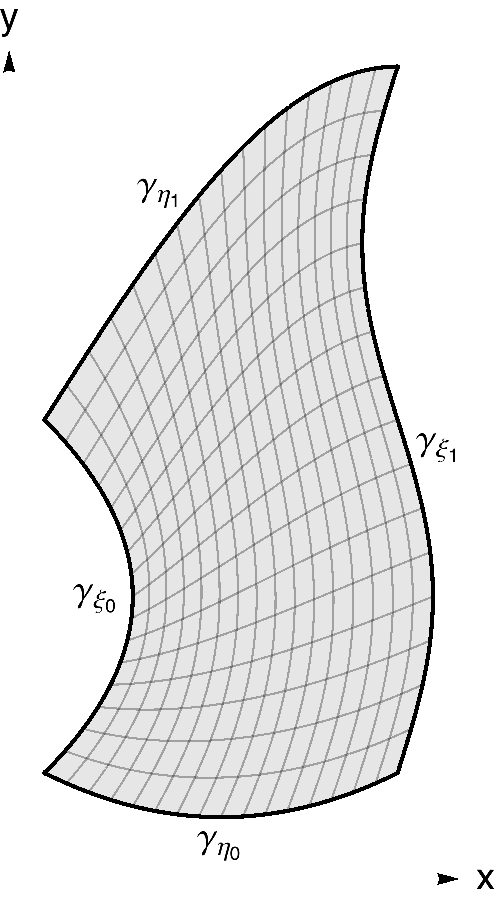
\includegraphics[width=.35\textwidth]{fig/testfig1.pdf}
\hspace{1cm}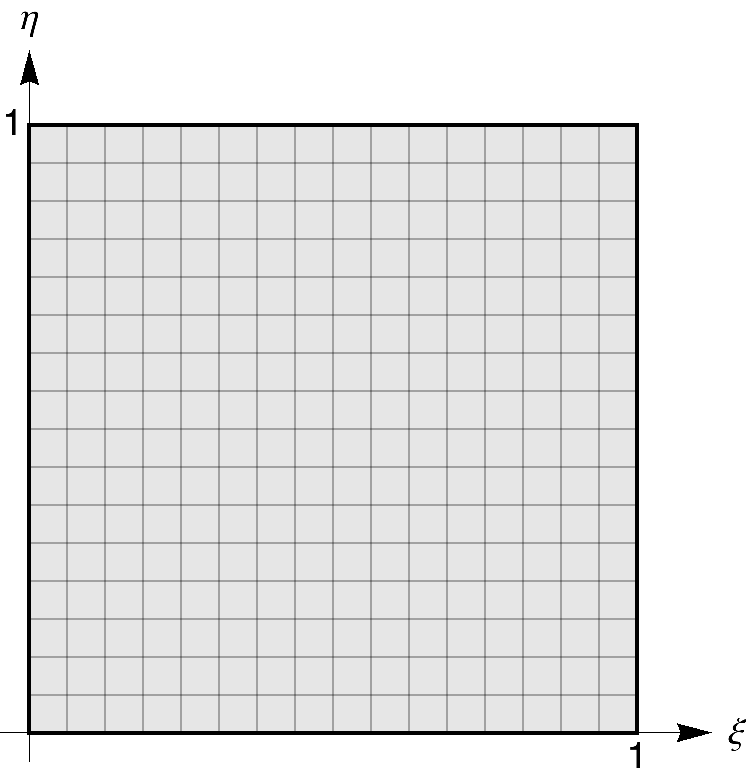
\includegraphics[width=.45\textwidth]{fig/testfig2.pdf}}
\caption{Figure Captions.}
\label{fig:label}
\end{figure}

\end{section}



%=== Appendix ============================================
\appendix

\dsp

\chapter{Appendix Title }{\label{appendix:a}}
\begin{section}{Section Title}

Appendicitis

\end{section}
\end{mainmatter}

%----- Bibliography ----------------
\ssp
\bibliographystyle{JHEP3}
\bibliography{dissertation}

\end{document} 
